\documentclass[english,hidelinks,pdftex, 11 pt, class=report,crop=false]{standalone}
\usepackage[T1]{fontenc}
\usepackage[utf8]{luainputenc}
\usepackage{lmodern} % load a font with all the characters
\usepackage{geometry}
\geometry{verbose,paperwidth=16.1 cm, paperheight=24 cm, inner=2.3cm, outer=1.8 cm, bmargin=2cm, tmargin=1.8cm}
\setlength{\parindent}{0bp}
\usepackage{import}
\usepackage[subpreambles=false]{standalone}
\usepackage{amsmath}
\usepackage{amssymb}
\usepackage{esint}
\usepackage{babel}
\usepackage{tabu}
\makeatother
\makeatletter

\usepackage{titlesec}
\usepackage{ragged2e}
\RaggedRight
\raggedbottom
\frenchspacing

% Norwegian names of figures, chapters, parts and content
\addto\captionsenglish{\renewcommand{\figurename}{Figur}}
\makeatletter
\addto\captionsenglish{\renewcommand{\chaptername}{Kapittel}}
\addto\captionsenglish{\renewcommand{\partname}{Del}}

\addto\captionsenglish{\renewcommand{\contentsname}{Innhold}}

\usepackage{graphicx}
\usepackage{float}
\usepackage{subfig}
\usepackage{placeins}
\usepackage{cancel}
\usepackage{framed}
\usepackage{wrapfig}
\usepackage[subfigure]{tocloft}
\usepackage[font=footnotesize,labelfont=sl]{caption} % Figure caption
\usepackage{bm}
\usepackage[dvipsnames, table]{xcolor}
\definecolor{shadecolor}{rgb}{0.105469, 0.613281, 1}
\colorlet{shadecolor}{Emerald!15} 
\usepackage{icomma}
\makeatother
\usepackage[many]{tcolorbox}
\usepackage{multicol}
\usepackage{stackengine}

% For tabular
\usepackage{array}
\usepackage{multirow}
\usepackage{longtable} %breakable table

% Ligningsreferanser
\usepackage{mathtools}
\mathtoolsset{showonlyrefs}

% index
\usepackage{imakeidx}
\makeindex[title=Indeks]

%Footnote:
\usepackage[bottom, hang, flushmargin]{footmisc}
\usepackage{perpage} 
\MakePerPage{footnote}
\addtolength{\footnotesep}{2mm}
\renewcommand{\thefootnote}{\arabic{footnote}}
\renewcommand\footnoterule{\rule{\linewidth}{0.4pt}}
\renewcommand{\thempfootnote}{\arabic{mpfootnote}}

%colors
\definecolor{c1}{cmyk}{0,0.5,1,0}
\definecolor{c2}{cmyk}{1,0.25,1,0}
\definecolor{n3}{cmyk}{1,0.,1,0}
\definecolor{neg}{cmyk}{1,0.,0.,0}

% Lister med bokstavar
\usepackage{enumitem}

\newcounter{rg}
\numberwithin{rg}{chapter}
\newcommand{\reg}[2][]{\begin{tcolorbox}[boxrule=0.3 mm,arc=0mm,colback=blue!3] {\refstepcounter{rg}\phantomsection \large \textbf{\therg \;#1} \vspace{5 pt}}\newline #2  \end{tcolorbox}\vspace{-5pt}}

\newcommand\alg[1]{\begin{align} #1 \end{align}}

\newcommand\eks[2][]{\begin{tcolorbox}[boxrule=0.3 mm,arc=0mm,enhanced jigsaw,breakable,colback=green!3] {\large \textbf{Eksempel #1} \vspace{5 pt}\\} #2 \end{tcolorbox}\vspace{-5pt} }

\newcommand{\st}[1]{\begin{tcolorbox}[boxrule=0.0 mm,arc=0mm,enhanced jigsaw,breakable,colback=yellow!12]{ #1} \end{tcolorbox}}

\newcommand{\spr}[1]{\begin{tcolorbox}[boxrule=0.3 mm,arc=0mm,enhanced jigsaw,breakable,colback=yellow!7] {\large \textbf{Språkboksen} \vspace{5 pt}\\} #1 \end{tcolorbox}\vspace{-5pt} }

\newcommand{\sym}[1]{\colorbox{blue!15}{#1}}

\newcommand{\info}[2]{\begin{tcolorbox}[boxrule=0.3 mm,arc=0mm,enhanced jigsaw,breakable,colback=cyan!6] {\large \textbf{#1} \vspace{5 pt}\\} #2 \end{tcolorbox}\vspace{-5pt} }

\newcommand\algv[1]{\vspace{-11 pt}\begin{align*} #1 \end{align*}}

\newcommand{\regv}{\vspace{5pt}}
\newcommand{\mer}{\textsl{Merk}: }
\newcommand\vsk{\vspace{11pt}}
\newcommand\vs{\vspace{-11pt}}
\newcommand\vsb{\vspace{-16pt}}
\newcommand\sv{\vsk \textbf{Svar:} \vspace{4 pt}\\}
\newcommand\br{\\[5 pt]}
\newcommand{\asym}[1]{../fig/#1}
\newcommand\algvv[1]{\vs\vs\begin{align*} #1 \end{align*}}
\newcommand{\y}[1]{$ {#1} $}
\newcommand{\os}{\\[5 pt]}
\newcommand{\prbxl}[2]{
\parbox[l][][l]{#1\linewidth}{#2
	}}
\newcommand{\prbxr}[2]{\parbox[r][][l]{#1\linewidth}{
		\setlength{\abovedisplayskip}{5pt}
		\setlength{\belowdisplayskip}{5pt}	
		\setlength{\abovedisplayshortskip}{0pt}
		\setlength{\belowdisplayshortskip}{0pt} 
		\begin{shaded}
			\footnotesize	#2 \end{shaded}}}

\renewcommand{\cfttoctitlefont}{\Large\bfseries}
\setlength{\cftaftertoctitleskip}{0 pt}
\setlength{\cftbeforetoctitleskip}{0 pt}

\newcommand{\bs}{\\[3pt]}
\newcommand{\vn}{\\[6pt]}
\newcommand{\fig}[1]{\begin{figure}
		\centering
		\includegraphics[]{\asym{#1}}
\end{figure}}
\newcommand{\net}[2]{{\color{blue}\href{#1}{#2}}}

\newcommand{\hrs}[2]{\hyperref[#1]{\color{blue}\textsl{#2 \ref*{#1}}}}
\newcommand{\rref}[1]{\hyperref[#1]{\color{blue}\textsl{Regel \ref*{#1}}}}

\newcommand{\sectionbreak}{\clearpage} % New page on each section

% Equation comments
\newcommand{\cm}[1]{\llap{\color{blue} #1}}

\newcommand\fork[2]{\begin{tcolorbox}[boxrule=0.3 mm,arc=0mm,enhanced jigsaw,breakable,colback=yellow!7] {\large \textbf{#1 (forklaring)} \vspace{5 pt}\\} #2 \end{tcolorbox}\vspace{-5pt} }


%%% SECTION HEADLINES %%%

% Our numbers
\newcommand{\likteikn}{Likhetstegnet}
\newcommand{\talsifverd}{Tall, siffer og verdi}
\newcommand{\koordsys}{Koordinatsystem}

% Calculations
\newcommand{\adi}{Addisjon}
\newcommand{\sub}{Subtraksjon}
\newcommand{\gong}{Multiplikasjon (Gonging)}
\newcommand{\del}{Divisjon (deling)}

%Factorization and order of operations
\newcommand{\fak}{Faktorisering}
\newcommand{\rrek}{Regnerekkefølge}

%Fractions
\newcommand{\brgrpr}{Introduksjon}
\newcommand{\brvu}{Verdi, utviding og forkorting av brøk}
\newcommand{\bradsub}{Addisjon og subtraksjon}
\newcommand{\brgngheil}{Brøk ganget med heltall}
\newcommand{\brdelheil}{Brøk delt med heltall}
\newcommand{\brgngbr}{Brøk ganget med brøk}
\newcommand{\brkans}{Kansellering av faktorer}
\newcommand{\brdelmbr}{Deling med brøk}
\newcommand{\Rasjtal}{Rasjonale tall}

%Negative numbers
\newcommand{\negintro}{Introduksjon}
\newcommand{\negrekn}{De fire regneartane med negative tall}
\newcommand{\negmeng}{Negative tall som mengde}

% Geometry 1
\newcommand{\omgr}{Begrep}
\newcommand{\eignsk}{Egenskaper for trekanter og firkanter}
\newcommand{\omkr}{Omkrets}
\newcommand{\area}{Areal}

%Algebra 
\newcommand{\algintro}{Introduksjon}
\newcommand{\pot}{Potenser}
\newcommand{\irrasj}{Irrasjonale tall}

%Equations
\newcommand{\ligintro}{Introduksjon}
\newcommand{\liglos}{Løsing ved de fire regneartene}
\newcommand{\ligloso}{Løsingsmetodene oppsummert}

%Functions
\newcommand{\fintro}{Introduksjon}
\newcommand{\lingraf}{Lineære funksjoner og grafer}

%Geometry 2
\newcommand{\geoform}{Formler for areal og omkrets}
\newcommand{\kongogsim}{Kongruente og formlike trekanter}
\newcommand{\geofork}{Forklaringar}

% Names of rules
\newcommand{\adkom}{Addisjon er kommutativ}
\newcommand{\gangkom}{Multiplikasjon er kommutativ}
\newcommand{\brdef}{Brøk som omskriving av delestykke}
\newcommand{\brtbr}{Brøk ganget med brøk}
\newcommand{\delmbr}{Brøk delt på brøk}
\newcommand{\gangpar}{Ganging med parentes (distributiv lov)}
\newcommand{\gangparsam}{Paranteser ganget sammen}
\newcommand{\gangmnegto}{Ganging med negative tall I}
\newcommand{\gangmnegtre}{Ganging med negative tall II}
\newcommand{\konsttre}{Konstruksjon av trekanter}
\newcommand{\kongtre}{Kongruente trekanter}
\newcommand{\topv}{Toppvinkler}
\newcommand{\trisum}{Summen av vinklene i en trekant}
\newcommand{\firsum}{Summen av vinklene i en firkant}
\newcommand{\potgang}{Ganging med potenser}
\newcommand{\potdivpot}{Divisjon med potenser}
\newcommand{\potanull}{Spesialtilfellet \boldmath $a^0$}
\newcommand{\potneg}{Potens med negativ eksponent}
\newcommand{\potbr}{Brøk som grunntall}
\newcommand{\faktgr}{Faktorer som grunntall}
\newcommand{\potsomgrunn}{Potens som grunntall}
\newcommand{\arsirk}{Arealet til en sirkel}
\newcommand{\artrap}{Arealet til et trapes}
\newcommand{\arpar}{Arealet til et parallellogram}
\newcommand{\pyt}{Pytagoras' setning}
\newcommand{\forform}{Forhold i formlike trekanter}
\newcommand{\vilkform}{Vilkår i formlike trekanter}
\newcommand{\omkrsirk}{Omkretsen til en sirkel (og $ \bm \pi $)}
\newcommand{\artri}{Arealet til en trekant}
\newcommand{\arrekt}{Arealet til et rektangel}
\newcommand{\liknflyt}{Flytting av ledd over likhetstegnet}
\newcommand{\funklin}{Lineære funksjoner}

%Opg
% Opg
\newcommand{\abc}[1]{
	\begin{enumerate}[label=\alph*),leftmargin=18pt]
		#1
	\end{enumerate}
}
\newcommand{\opgt}{\phantomsection \addcontentsline{toc}{section}{Oppgaver} \section*{Oppgaver for kapittel \thechapter}\vs \setcounter{section}{1}}
\newcounter{opg}
\numberwithin{opg}{section}
\newcommand{\op}[1]{\vspace{15pt} \refstepcounter{opg}\large \textbf{\color{blue}\theopg} \vspace{2 pt} \label{#1} \\}
\newcommand{\ekspop}{\vsk\textbf{Gruble \thechapter}\vspace{2 pt} \\}
\newcommand{\nes}{\stepcounter{section}
	\setcounter{opg}{0}}
\newcommand{\opr}[1]{\vspace{3pt}\textbf{\ref{#1}}}

%License
\newcommand{\lic}{\textit{Matematikken sine byggesteiner by Sindre Sogge Heggen is licensed under CC BY-NC-SA 4.0. To view a copy of this license, visit\\ 
		\net{http://creativecommons.org/licenses/by-nc-sa/4.0/}{http://creativecommons.org/licenses/by-nc-sa/4.0/}}}

\usepackage{datetime2}
\usepackage[]{hyperref}


\begin{document}
\section{Addisjon}

\subsubsection{Oppstilling}
Denne metoden baserer seg på plassverdisystemet, der man trinnvis regner ut summen av enerne, tierne, hundrene, o.l.
\begin{center}
	\parbox{0.3\linewidth}{
\eks[1]{
	\begin{figure}
		\centering
		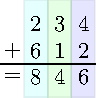
\includegraphics[]{rekfig/plus1}
	\end{figure}
}
}\qquad
\parbox{0.3\linewidth}{
\eks[2]{
	\begin{figure}
		\centering
		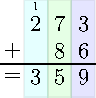
\includegraphics[]{rekfig/plus2}
	\end{figure}
}
}\\[12pt]
\parbox{0.3\linewidth}{
\eks[3]{
	\begin{figure}
		\centering
		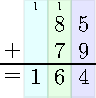
\includegraphics[]{rekfig/plus3}
	\end{figure}
}}\qquad
\parbox{0.3\linewidth}{
\eks[4]{
	\begin{figure}
		\centering
		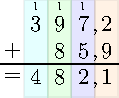
\includegraphics[]{rekfig/plus4}
	\end{figure}
}}
\end{center}
\fork{Eksempel 1}{
\begin{figure}
	\centering
	\subfloat[]{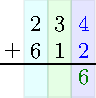
\includegraphics{rekfig/plus1a}}\qquad
	\subfloat[]{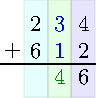
\includegraphics{rekfig/plus1b}}\qquad
	\subfloat[]{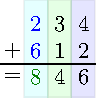
\includegraphics{rekfig/plus1c}}
\end{figure}

\begin{enumerate}[label=\alph*)]
	\item Vi legger sammen enerne: $ 4+2=6 $
	\item Vi legger sammen tierne: $ 3+1=4 $
	\item Vi legger sammen hundrene: $ 2+6=8 $
\end{enumerate}
} \newpage
\fork{Eksempel 2}{
	\begin{figure}
		\centering
		\subfloat[]{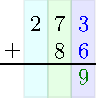
\includegraphics{rekfig/plus2a}}\qquad
		\subfloat[]{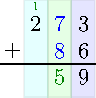
\includegraphics{rekfig/plus2b}}\qquad
		\subfloat[]{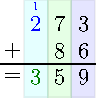
\includegraphics{rekfig/plus2c}}
	\end{figure}
	
	\begin{enumerate}[label=\alph*)]
		\item Vi legger sammen enerne: $ 3+6=9 $
		\item Vi legger sammen tierne: $ {7+8=15} $. Siden 10 tiere er det samme som 100, legger vi til 1 på hundreplassen, og skriver opp de resterende 5 tierne på tierplassen.
		\item Vi legger sammen hundrene: $ 1+2=3 $.
	\end{enumerate}
} \vsk

\spr{
Det å skrive 1 på neste sifferplass kalles ''å skrive 1 i mente''.
}
\subsubsection{Tabellmetoden}
Denne metoden tar utgangspunkt i det éne leddet, og summerer fram til det andre leddet er nådd. Det som i starten kan være litt rart med denne metoden, er at du selv velger fritt hvilke tall du skal legge til, så lenge du når det andre leddet til slutt.
\begin{center}
	\parbox{0.3\linewidth}{
		\eks[1]{
			$ \colb{273}+\colc{86} = \colo{359} $ \vsk
			
			\begin{tabular}{r|r|r}
				&&\colb{273} \\ \hline
				6 & 6 & 279 \\
				30& 36 & 309 \\
				50& \colc{86} & \colo{359}
			\end{tabular}
		}
	} \qquad
	\parbox{0.3\linewidth}{
		\eks[2]{
			$ \colb{85}+\colc{79}=\colo{164} $  \vsk
			
			\begin{tabular}{r|r|r}
				& & \colb{85} \\ \hline 
				5 & 5 & 90 \\
				10 & 15 &100 \\
				64 & \colc{79} & \colo{164} \\
			\end{tabular} \vsk
		}
	}
\end{center}
\newpage
\fork{Eksempel 1}{
\begin{figure}
	\centering
\subfloat[]{
\begin{tabular}{r|r|r}
	&&\colb{273} \\ \hline
	 &  &  \\
	\phantom{30}& \phantom{36} &  \\
	&  & 
\end{tabular}
} \qquad
\subfloat[]{
	\begin{tabular}{r|r|r}
		&&\colb{273} \\ \hline
		6& 6 & 279 \\
		\phantom{30}& \phantom{36} &  \\
		&  & 
	\end{tabular}
}\vsk 

\subfloat[]{
	\begin{tabular}{r|r|r}
		&&\colb{273} \\ \hline
		6& 6 & 279 \\
		30& 36 & 309  \\
		&  & 
	\end{tabular}
}
\qquad
\subfloat[]{
	\begin{tabular}{r|r|r}
		&&\colb{273} \\ \hline
		6& 6 & 279 \\
		30& 36 & 309  \\
		50& \colc{86} & \colo{359}
	\end{tabular}
}
\end{figure}
\begin{enumerate}[label=(\alph*)]
\item Vi starter med det leddet vi selv ønsker, ofte er det lurt å starte med det største leddet.
\item Vi legger til $ 6 $. Da har vi totalt lagt til $ 6 $, og videre er $ {273+6=279} $.
\item Vi legger til 30. Da har vi totalt lagt til 36, og videre er $ 279+30=309 $.
\item Vi legger til 50. Da har vi totalt lagt til 86, altså har vi nådd det andre leddet, og videre er $ 309+50=359 $.
\end{enumerate}
} \vsk

\info{Oppstilling versus tabellmetoden}{
	Ved første øyekast kan kanskje tabellmetoden bare se ut som en innviklet måte å regne addisjon på samenlignet med oppstilling, men med øving vil mange oppdage at tabellmetoden bedrer evnen til hoderegning. 
}

\section{Subtraksjon}
\subsubsection{Oppstilling}
Subtraksjon med oppstilling baserer seg på plassverdisystemet, der man trinnvis regner differansen mellom enerne, tierne, hundrene, o.l. Metoden tar også utgangspunkt i et mengdeperspektiv, og tillater derfor ikke differanser med negativ verdi (se forklaringen til \textsl{Eksempel 2}).
\begin{center}
	\parbox{0.3\linewidth}{
\eks[1]{
	\begin{figure}
		\centering
		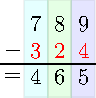
\includegraphics[]{rekfig/min1}
	\end{figure}
}} \qquad
\parbox{0.3\linewidth}{
\eks[2]{
	\begin{figure}
		\centering
		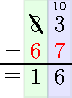
\includegraphics[]{rekfig/min2}
	\end{figure}
}} \\[12pt]
\parbox{0.3\linewidth}{
\eks[3]{
	\begin{figure}
		\centering
		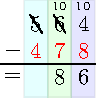
\includegraphics[]{rekfig/min3}
	\end{figure}
}}\qquad
\parbox{0.3\linewidth}{
\eks[4]{
	\begin{figure}
		\centering
		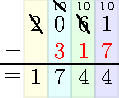
\includegraphics[]{rekfig/min4}
	\end{figure}
}}

\end{center}
\fork{Eksempel 1}{ \vs
\begin{figure}
	\centering
	\subfloat[]{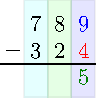
\includegraphics{rekfig/min1a}}\qquad
	\subfloat[]{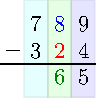
\includegraphics{rekfig/min1b}}\qquad
	\subfloat[]{
\includegraphics{rekfig/min1c}}
\end{figure}

\begin{enumerate}[label=(\alph*)]
	\item Vi finner differansen mellom enerne: $ {9-4=5} $
	\item Vi finner differansen mellom tierne: $ {8-2=6} $. 
	\item Vi finner differansen mellom hundrene: $ {7-3=4} $.
\end{enumerate}
}
\newpage
\fork{Eksempel 2}{ \vs
	\begin{figure}
		\centering
		\subfloat[]{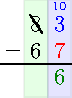
\includegraphics{rekfig/min2a}}\qquad
		\subfloat[]{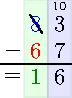
\includegraphics{rekfig/min2b}}
	\end{figure}
	
	\begin{enumerate}[label=(\alph*)]
		\item Vi merker oss at 7 er større enn 3, derfor tar vi 1 tier fra de 8 på tierplassen. Dette markerer vi ved å sette en strek over 8. Så finner vi differansen mellom enerne: $ {13-7=6} $
		\item Siden vi tok 1 fra de 8 tierne, er der nå bare 7 tiere. Vi finner differansen mellom tierne: $ {7-6=1} $.
	\end{enumerate}
}
\subsubsection{Tabellmetoden}
Tabellmetoden for subtraksjon tar utgangspunkt i at subtraksjon er en omvendt operasjon av addisjon. For eksempel, svaret på spørsmålet ''Hva er $ 789-324 $?'' er det samme som svaret på spørsmålet ''Hvor mye må jeg legge til på 324 for å få 789?''. Med tabellmetoden følger du ingen spesiell regel underveis, men velger selv tallene du mener passer best for å nå målet.\\
\begin{center}
\parbox{0.35\linewidth}{
\eks[1]{
$ \colb{789}-\colr{324}=\colc{465} $	 \vsk

\begin{tabular}{r|r}
	& \colr{324} \\ \hline
	6&330 \\
	70&400 \\
	389&\colb{789} \\ \hline
	\colc{465}
\end{tabular}
}} \qquad
\parbox{0.35\linewidth}{
	\eks[2]{
		$ \colb{83}-\colr{67}=\colc{16} $	 \vsk
		
		\begin{tabular}{r|r}
			& \colr{67} \\ \hline
			3&70 \\
			13&\colb{83} \\ \hline
			\colc{16}
		\end{tabular} \vspace{14pt}
}} \\[12pt]
\parbox{0.35\linewidth}{
	\eks[3]{
		$ 564-478=86 $\vsk
		
		\begin{tabular}{r|r}
			& 478 \\ \hline
			2&480 \\
			20&500 \\ 
			64&564\\ \hline
			86
		\end{tabular}
}} \qquad 
\parbox{0.4\linewidth}{
	\eks[4]{
		$ {206,1-31,7=174,4} $\vsk
		
		\begin{tabular}{r|r}
			& 31,7 \\ \hline
			0,3& 32\phantom{,0} \\
			70\phantom{,0}&102\phantom{,0} \\ 
			104,1&206,1\\ \hline
			174,4
		\end{tabular}
}}
\end{center}
\fork{Eksempel 1}{
	\[ \colb{789}-\colr{324}=\colo{465} \]
\begin{figure}
	\centering
	\subfloat[]{
	\begin{tabular}{r|r}
		& \colr{324} \\ \hline
		& \\
		& \\
		& \\ \hline
		&
	\end{tabular}	
} \qquad
	\subfloat[]{
	\begin{tabular}{r|r}
		& \colb{324} \\ \hline
	   \colb{6}& \colc{330}\\
		& \\
		& \\ \hline
		&
	\end{tabular}
}\qquad
	\subfloat[]{
	\begin{tabular}{r|r}
		& 324 \\ \hline
		6& \colb{330}\\
		\colb{70}& \colc{400} \\
		& \\ \hline
		&
	\end{tabular}	
}  \\[12pt]
\subfloat[]{
	\begin{tabular}{r|r}
		& 324 \\ \hline
		6& 330\\
		70& \colb{400} \\
		\colb{389}& \colc{789}\\ \hline
		&
	\end{tabular}	
}\qquad
\subfloat[]{
	\begin{tabular}{r|r}
		& 324 \\ \hline
		\colb{6}& 330\\
		\colb{70}& 400 \\
		\colb{389}& 789\\ \hline
		\colo{465}&
	\end{tabular}	
}
\end{figure}
\begin{enumerate}[label=(\alph*)]
	\item Vi starter med 324.
	\item Vi legger til 6, og får $ {324+6=330} $
	\item Vi legger til 70, og får $ {70+330=400} $
	\item Vi legger til 389, og får $ {389+400=789} $. Da er vi framme på 789.
	\item Vi summerer tallene vi har lagt til:  $ {6+70+389=465} $
\end{enumerate}
}
\section{Ganging} \label{rekGanging}
\subsubsection{Ganging med 10, 100, 1\,000 osv.}
\reg[Å gange heltall med 10, 100 osv. \label{gangheltallmed10100}]{
	\vs
	\begin{itemize}
		\item Når man ganger et heltall med 10, får man svaret ved å legge til sifferet 0 bak heltallet.
		\item Når man ganger et heltall med 100, får man svaret ved å legge til sifrene 00 bak heltallet.
		\item Det samme mønsteret gjelder for tallene 1\,000, 10\,000 osv.
	\end{itemize}
}
\eks[1]{\vsb \vsb
	\alg{
		6\cdot \colb{10} &= 6\colb{0}\vn
		79\cdot \colb{10} &= 79\colb{0} \vn
		802\cdot\colb{10}&=802\colb{0}
	}
}
\eks[2]{ \vsb \vsb
\alg{ 
6\cdot\colb{100} &= 6\colb{00} \vn
79\cdot\colb{100} &= 7\,9\colb{00} \vn
802\cdot\colb{100} &=80\,2\colb{00}
}
}
\eks[3]{ \vsb \vsb
\alg{ 
	6\cdot\colb{1\,000} &= 6\,\colb{000} \vn
	79\cdot\colb{10\,000} &= 79\colb{0\,000} \vn
	802\cdot\colb{100\,000} &=80\,2\colb{00\,000}
}
}
\newpage
\reg[Å gange desimaltall med 10, 100 osv. \label{gangdesmed10100}]{
	\vs
	\begin{itemize}
		\item Når man ganger et desimaltall med 10, får man svaret ved å flytte komma en plass til høgre.
		\item Når man ganger et heltall med 100, får man svaret ved å flytte komma to plasser til høgre.
		\item Det samme mønsteret gjelder for tallene 1\,000, 10\,000 osv.
	\end{itemize}
}
\eks[1]{\vsb \vsb
	\alg{
		7\colr{,}9\cdot 10 &= 79\colr{,}=79 \vn
		38\colr{,}02\cdot10&=380\colr{,}2 \vn
		0\colr{,}57\cdot 10 &=05\colr{,}7=5\colr{,}7 \vn
		0\colr{,}194\cdot 10&= 01\colr{,}94=1\colr{,}94
	}
}
\eks[2]{ \vsb \vsb
	\alg{
		7\colr{,}9\cdot 100 &= 790\colr{,}=790 \vn
		38\colr{,}02\cdot100&=3802\colr{,}=3\,802 \vn
		0\colr{,}57\cdot 100 &=057\colr{,}=57 \vn
		0\colr{,}194\cdot 100&= 019\colr{,}4=19\colr{,}4
	}
}
\eks[3]{ \vsb \vsb
	\alg{
	7\colr{,}9\cdot 1\,000 &= 7900\colr{,}=7\,900 \vn
	38\colr{,}02\cdot10\,000&=38020\colr{,}=38\,020 \vn
	0\colr{,}57\cdot 100\,000 &=05\colr{,}7=57000\colr{,}=57\,000
}
}
\info{Merk}{
\rref{gangheltallmed10100} er bare et spesialtilfelle av \rref{gangdesmed10100}. For eksempel, å bruke \rref{gangheltallmed10100} på regnestykket $ {7\cdot 10} $ gir samme resultat som å bruke \rref{gangdesmed10100} på regnestykket $ {7,0\cdot 10} $. 
}
\newpage
\fork{Å gange tall med 10, 100 osv.}{
Titallsystemet baserer seg på grupper av ti, hundre, tusen osv., og tideler, hundredeler og tusendeler osv (se \rref{titalsys}). Når man ganger et tall med 10, vil alle enere i tallet bli til tiere, alle tiere bli til hundrere osv. Hvert siffer forskyves altså én plass mot venstre. Tilsvarende forskyves hvert siffer to plasser mot venstre når man ganger med 100, tre plasser når man ganger med 1\,000 osv.
}
\subsubsection{Utvidet form}
Ganging på utvidet form bruker vi for å regne multiplikasjon mellom flersifrede tall. Metoden baserer seg på distributiv lov (\rref{gangpar}). \regv
\eks[1]{ \vs
\begin{figure}
	\centering
	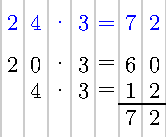
\includegraphics[]{rekfig/gang1}
\end{figure}
}
\eks[2]{ \vs
\begin{figure}
	\centering
	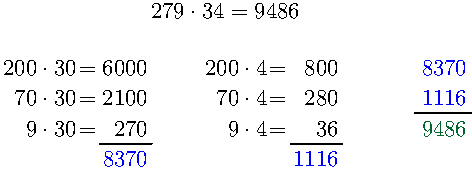
\includegraphics[]{rekfig/gfleirsif}
\end{figure}
}
\fork{Eksempel 1}{
24 kan skrives som $ 20+4 $, altså er
\[ 24\cdot3 =(20+4)\cdot3 \]
Videre er 
\algv{
(20+4)\cdot 3 &=20\cdot 3 + 4\cdot 3 \\
&= 60+12 \\
&= 72
}
}
\newpage
\fork{Eksempel 2}{
Vi har at
\alg{
279&=200+70+9 \\
34 &=30+4 	
}
Altså er
\alg{
279\cdot34&= (200+70+9)\cdot (30+4) 
}
Videre er 
{
\footnotesize
\alg{
(200+70+9)\cdot (30+4) &=200\cdot 30+70\cdot30+9\cdot30+200\cdot4+70\cdot4+9\cdot4
\\
&=9486}
} \vs
}
\subsubsection{Kompaktmetoden}
Kompaktmetoden bygger på de samme prinsippene som ganging på utvidet form, men har en skrivemåte som gjør utregningen korterere. \regv

\eks[1]{
	\begin{figure}
		\centering
		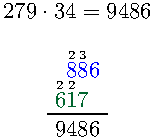
\includegraphics[]{rekfig/gfleirsifa}
	\end{figure}
}
\newpage
\fork{Eksempel 1}{
Vi starter med å gange sifrene i 279 enkeltvis med 4:
\begin{itemize}
	\item $ 9\cdot 6=36 $, da skriver vi 6 på enerplassen og 3 i mente.
	\item $ 7\cdot4 =28$, da skriver vi 8 på tierplassen og 2 i mente.
	\item $ 2\cdot 4=8 $, da skriver vi 8 på hundrerplassen.
\end{itemize}
Så ganger vi sifrene i 279 enkeltvis med 30. Dette kan forenkles til å gange med 3, så lenge vi plasserer sifrene én plass forskjøvet til venstre i forhold til da vi ganget med 4:
\begin{itemize}
	\item $ 9\cdot 3=27 $, da skriver vi 7 på tierplassen og 2 i mente. 
	\item $ 7\cdot3=21 $, da skriver vi 1 på hundrerplassen og 2 i mente.
	\item $ 2\cdot3=6 $, da skriver vi 6 på tusenplassen.
\end{itemize} 
}
\section{Divisjon} \label{rekDivisjon}
\subsubsection{\delmedtihundre}
\reg[Deling med 10, 100, 1\,000 osv. \label{deledesmed10100}]{ \vs
\begin{itemize}
	\item Når man deler et desimaltall med 10, får man svaret ved å flytte komma en plass til venstre.
	\item Når man deler et desimaltall med 10, får man svaret ved å flytte komma to plasser til venstre.
	\item Det samme mønsteret gjelder for tallene 1\,000, 10\,000 osv.
\end{itemize}
}
\eks[1]{ \vsb \vsb
	\alg{
200:10&=200\colr{,}0:10 \\&=20\colr{,}00\\&=20	\vn
45:10&=45\colr{,}0:10 \\&= 4\colr{,}50 \\&=4\colr{,}5
}
}
\eks[2]{ \vsb \vsb
	\alg{
		200:100&=200\colr{,}0:100 \\&=2\colr{,}000\\&=2	\vn
		45:100&=45\colr{,}0:100 \\&= 0\colr{,}450 \\&=0\colr{,}45
	}
}
\newpage
\eks[3]{ \vsb \vsb
\alg{
143\colr{,}7 :10 &= 14\colr{,}37 \vn
143\colr{,}7 :100 &= 1\colr{,}437 \vn
143\colr{,}7 :1\,000 &= 0\colr{,}1437 \vn
93\colr{,}6:10 &= 9\colr{,}36 \vn
93\colr{,}6:100 &= 0\colr{,}936 \vn
93\colr{,}6:1\,000 &= 0\colr{,}0936
}
}
\fork{Deling med 10, 100, 1\,000 osv.}{
Titallsystemet baserer seg på grupper av ti, hundre, tusen osv., og tideler, hundredeler og tusendeler osv (se \rref{titalsys}). Når man deler et tall med 10, vil alle enere i tallet bli til tideler, alle tiere bli til enere osv. Hvert siffer forskyves altså én plass mot høgre. Tilsvarende forskyves hvert siffer to plasser mot høgre når man deler med 100, tre plasser når man deler med 1\,000 osv.
}

\subsubsection{Oppstilling}
Divisjon med oppstilling baserer seg på divisjon tolket som inndeling av mengder (se s. \pageref{Divisjon})

\begin{center}
	\parbox{0.3\linewidth}{
	\eks[1]{ \vsb
		\begin{figure}
			\centering
			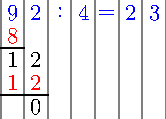
\includegraphics[]{rekfig/del1}
		\end{figure} \vspace{18pt}
	}
}\qquad
\parbox{0.45\linewidth}{
	\eks[1]{ \vspace{-5pt}
		\begin{figure}
			\centering
			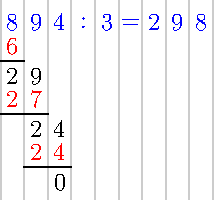
\includegraphics[]{rekfig/del2}
		\end{figure}
	}
}
\end{center}
\newpage
\fork{Eksempel 1}{ \vs \vs
	\begin{figure}
		\centering
		\subfloat{\includegraphics{\asym{delalg}}}
		\qquad \subfloat{\includegraphics[angle=90]{\asym{delalg0}}}
	\end{figure}
	Figuren over illustrerer mengden 92, som vi skal dele inn i 4 like store grupper. 
	\begin{itemize}
		\item Vi starter med å fordele så mange av tierne som mulig. Av de 9 tierne, kan hver gruppe få 2. Da har vi totalt fordelt $ 2\cdot 4=8 $ tiere.
		\begin{figure}
			\centering
			\subfloat{\includegraphics{\asym{delalgaa}}}
			\qquad \subfloat{\includegraphics[angle=90]{\asym{delalga}}}
		\end{figure}
		\item Vi står nå igjen med 1 tier og 2 enere, altså 12 enere. Av de 12 enerne, kan hver gruppe få 3. Da har vi totalt fordelt $ 3\cdot 4= 12 $ enere.
		\begin{figure}
			\centering
			\includegraphics[angle=90]{\asym{delalgb}}
		\end{figure}
		\item Nå er hele mengden 92 fordelt, og da er vi ferdige med utregningen. I hver gruppe endte vi opp med mengden 23.
	\end{itemize}
}
\newpage
\subsubsection{Tabellmetoden}
Tabellmetoden baserer seg på divisjon som omvendt operasjon av ganging. For eksempel er svaret på spørsmålet ''Hva er $ {76:4} $'' det samme som svaret på spørsmålet ''Hvilket tall må jeg gange 4 med for å få 76?''. På samme vis som for tabellmetoden ved subtraksjon er det opp til en selv å velge passende tall for å nå målet.
\begin{center}
	\parbox{0.35\linewidth}{
		\eks[1]{
			$ \colg{76}:\colb{4}=\colo{19} $	 \vsk
			
			\begin{tabular}{r|r|r}
				$ \cdot\, \colb{4} $&\\ \hline
				10&40&40 \\
				9& 36 &\colg{76} \\ \hline
				\colo{19}&
			\end{tabular}
		\vspace{42pt}
	}} \qquad
\parbox{0.35\linewidth}{
	\eks[2]{
		$ \colg{894}:\colb{3}=\colo{298} $	 \vsk
		
		\begin{tabular}{r|r|r}
			$ \cdot\, \colb{3} $&\\ \hline
			200& 600 &600 \\
			30&90 &690 \\
			30&90 &780 \\
			30& 90&870 \\
			8&24 &\colg{894} \\ \hline
			\colo{298} &
		\end{tabular}
}} \vsk

\parbox{0.415\linewidth}{
	\eks[3]{		
		$ 894:3=298 $	 \vsk
		
		\begin{tabular}{r|r|r}
			$ \cdot\, 3 $&\\ \hline
			300& 900&900 \\
			$ -2 $& $ -6 $ &894 \\ \hline
			298&
		\end{tabular} \vsk
	
\footnotesize	
\mer Samme regnestykke som i \textsl{Eksempel 2}, men en annen utregning.
}
}
\end{center}
\newpage
\fork{Eksempel 1}{
	Siden vi skal dele \colg{92} med \colb{4}, gangar vi med \colb{4} fram til vi når \colg{92}.
	\begin{figure}
		\centering
		\subfloat[]{
			\begin{tabular}{r|r|r}
				$ \cdot\, \colb{4} $&\\ \hline
				10&40&40 \\
				&& \\
				& &\\ \hline
				&
			\end{tabular}	
		} \qquad
		\subfloat[]{
			\begin{tabular}{r|r|r}
				$ \cdot\, \colb{4} $&\\ \hline
				10&40&40 \\
				10&40&80 \\
				&  & \\ \hline
				&
			\end{tabular}	
		} \\
		\subfloat[]{
			\begin{tabular}{r|r|r}
				$ \cdot\, \colb{4} $&\\ \hline
				10&40&40 \\
				10&40&80 \\
				3& 12 &\colg{92} \\ \hline
				&
			\end{tabular}	
		} \qquad
		\subfloat[]{
			\begin{tabular}{r|r|r}
				$ \cdot\, \colb{4} $&\\ \hline
				10&40&40 \\
				10&40&80 \\
				3& 12 &\colg{92} \\ \hline
				\colo{23}&
			\end{tabular}	
		}
	\end{figure}
	\begin{enumerate}[label=(\alph*)]
		\item Vi ganger 10 med 4, som er lik 40. Da har vi så langt kommet til 40.
		\item Vi ganger 10 med 4, som er lik 40. Da har vi så langt kommet til $ {40+40=80} $.
		\item Vi ganger 3 med 4, som er lik 12. Da har vi kommet til $ {80+12=92} $, som var målet.
		\item Vi legger sammen tallene vi ganget med, og får $ {10+10+3=23} $.
	\end{enumerate}
}
\info{Tips}{
	Det kan være lurt å se tilbake på utregninger gjort med tabellmetoden for å tenke over om man kunne valgt tall på en bedre måte. For eksempel, i \textsl{Eksempel 1} over kunne vi startet med å gange med 20. Dette er omtrent like enkelt som å gange med 10, og det ville ha brakt oss nærmere målet.
}
\newpage
\subsubsection{Divisjon med rest}
Det er langt ifra alltid at svaret ved divisjon blir et heiltal. En måte å uttrykke slike svar på, er å ved å bruke begrepet \textit{rest}\index{rest}. Begrepet er best forklart ved eksempel: \regv
\eks[1]{
	Regn ut $ 11:4 $ med rest.
	
	\sv
	Det største heltallet vi kan gange med 4 uten at produktet blir større enn
	11, er 2. $ {2\cdot 4 = 8} $, så da har vi $ 11-8=3 $ i rest.
	\[ 11= \colb{2}\cdot 4 +\colc{3} \]	
	\fig{mod1}
	Dette betyr at
	\[ 11:4 =\text{\colb{2} og \colc{3} i rest}\]
}
\eks[2]{
	Regn ut $ 19:3 $ med rest.
	
	\sv
	Det største heltallet vi kan gange med 3 uten at produktet blir større enn
	19, er 6. $ {6\cdot 3 = 18} $, så da har vi $ 19-8=1 $ i rest.
	\[ 19= \colb{6}\cdot 3 +\colc{1} \]	
	\fig{mod2}
	Dette betyr at
	\[ 19:3 =\text{\colb{6} og \colc{1} i rest}\]
}
\newpage
\eks[3]{
	Regn ut $ 94:4 $ med rest.
	
	\sv
	\metode{Med oppstilling}{3.75cm}
	\[ 94:4 = \text{23 og 2 i rest} \]
	\begin{figure}
		\centering
		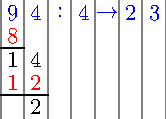
\includegraphics[]{rekfig/mod3}
	\end{figure}
	\mers{Da det blir feil å bruke \sym{$ = $} i figuren over, har vi valgt å bruke \sym{$  \rightarrow$}. 
	}\vsk 
	
	\metode{Med tabellmetoden}{3.75cm}
	\[ 94:4 = \text{23 og 2 i rest} \]
	\begin{center}
		\begin{tabular}{r|r|r}
			$ \cdot\, 4$&\\ \hline
			20&80&80 \\
			3& 12 &92 \\ \hline
			23&
		\end{tabular} \qquad $ 94-92=2 $
	\end{center}
}
\spr{
	Hvis vi utfører en \textit{modulo-operasjon}, finner vi resten i et delestykke. Dette blir ofte vist ved forkortingen \sym{mod}. For eksempel er
	\[ 11\text{ mod } 4= 3\qquad , \qquad 19\text{ mod 3} =1 \]
	I tillegg til \sym{\texttt{mod}}, blir også \sym{\texttt{\%}} og \sym{{\texttt{\string \\}}} brukt som symbol for denne operasjonen i programmeringsspråk.
}
\newpage
\subsubsection{Divisjon med blanda tall som svar}
\eks[1]{
	Regn ut $ 11:4 $. Skriv svaret som et blandet tall.
	
	\sv \vsb
	\[ 11:4 = \text{2 og 3 i rest}=2+\frac{3}{4} \]
}
\eks[2]{
	Regn ut $ 19:3 $. Skriv svaret som et blandet tall.
	
	\sv \vsb
	\[ 19:3=\text{6 og 1 i rest}=6+\frac{1}{3} \]
}
\fork{Eksempel 1}{
	Vi starter med å legge merke til at $ 4=\frac{4}{1} $. Dette betyr at
	\[ 11:4 = 11:\frac{4}{1} \]
	Av \rref{delmbr} har vi at
	\[ 11:\frac{4}{1} = 11\cdot \frac{1}{4} \]
	Videre er $ 11=2\cdot 4+ 3 $, og da er
	\[ 11\cdot \frac{1}{4}=(2\cdot 4+3)\cdot\frac{1}{4} \]
	Av \rref{gangpar} har vi at
	\alg{
		(2\cdot 4+3)\cdot\frac{1}{4}&=2\cdot4\cdot\frac{1}{4}+3\cdot \frac{1}{4} \\
		&= 2+\frac{3}{4}
	}
}
\newpage
\subsection{Divisjon med desimaltall som svar}
\eks[1]{
	Regn ut $ 11:4 $. Oppgi svaret som desimaltal.
	
	\sv
	
	\metode{Med oppstilling}{3.75cm} \vs
	\[ 11:4=2,75 \]
	\begin{figure}
		\centering
		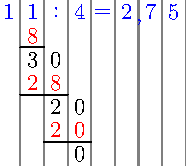
\includegraphics{rekfig/deldes1}
	\end{figure}
	\metode{Med tabellmetoden}{3.75cm} \vs
	\[ 11:4 = 2,75\]
	\begin{center}
		\begin{tabular}{r|r|r}
			$ \cdot\, 4$&\\ \hline
			2&8&8 \\
			0,5& 2 &10 \\
			0,25& 1 &11\\ \hline
			2,75&
		\end{tabular}
	\end{center}
}
\fork{Eksempel 1; oppstilling}{
	Siden vi deler med 4, er det snakk om å fordele 11 likt i 4 grupper.
	\begin{itemize}
		\item 8 av de 11 enerne kan vi fordele likt i 4 grupper. Da har vi igjen 3 enere. Dette er det samme som 30 tideler.
		\item 28 av de 30 tidelene kan vi fordele likt i 4 grupper. Da har vi igjen 2 tideler. Dette er det samme som 20 hundredeler.
		\item 20 av de 20 hundredelene kan vi fordele likt i 4 grupper.
		\item Hele mengden 11 er nå fordelt, og da er vi ferdige med utegningen.
	\end{itemize}
}
\newpage
\section{Primtalsfaktorisering \label{primtalsfakt}}
\mer Primtala mellom 1-100 finn du på side \pageref{primtalfig}.


\begin{center}
	\parbox{0.35\linewidth}{
		\eks[1]{
			$ \colo{84}= \colb{2\cdot2\cdot3\cdot7}$	 \vsk
			
			\begin{tabular}{r|r|r}
				& $ : $&\\ \hline
				\colo{84}&\colb{2}&\colg{42} \\
				\colg{42}& \colb{2} &\colg{21} \\ 
				\colg{21}&\colb{3}&\colb{7}\\
				\hline
			\end{tabular}
	}} \qquad
	\parbox{0.35\linewidth}{
		\eks[2]{
			$ \colo{595}= \colb{5\cdot7\cdot17}$	 \vsk
			
			\begin{tabular}{r|r|r}
				& $ : $&\\ \hline
				\colo{595}& \colb{5} &\colg{119} \\ 
				\colg{119}&\colb{7}&\colb{17}\\
				\hline
			\end{tabular}
			\vspace{12pt}
	}}
\end{center} 


\fork{Eksempel 1}{ \vs
	\begin{figure}
		\centering
		\subfloat[]{
			\begin{tabular}{r|r|r}
				& $ : $&\\ \hline
				\colo{84}&\colb{2}&\colg{42} \\
				&& \\ 
				&&\\
				\hline
			\end{tabular}
		} \qquad
		\subfloat[]{
			\begin{tabular}{r|r|r}
				& $ : $&\\ \hline
				\colo{84}&\colb{2}&\colg{42} \\
				\colg{42}& \colb{2} &21 \\ 
				&&\\
				\hline
			\end{tabular}
		}\vsk 
		
		\subfloat[]{
			\begin{tabular}{r|r|r}
				& $ : $&\\ \hline
				\colo{84}&\colb{2}&42 \\
				42& \colb{2} &\colg{21} \\ 
				\colg{21}&\colb{3}&\colb{7}\\
				\hline
			\end{tabular}
		}
	\end{figure}
	\begin{enumerate}[label=(\alph*)]
		\item Sidan 2 er det første primtallet, undersøker vi om 84 er deleleg med 2. Det er det, fordi $ 84:2=42 $.
		\item Vi undersøker om også 42 er deleleg med 2. Det er det, fordi $ 42:2=21 $.
		\item Vi undersøker om også 21 er deleleg med 2. Det er det ikkje, fordi $ {21:2=10,5} $. Derfor går vi over til neste primtall, som er 3. 21 er deleleg med 3 fordi $ 21:3=7 $.
	\end{enumerate}
	Sidan 7 er eit primtal, er vi komme i mål.
}
\newpage
\label{primtalfig}
\fig{primn100}

\end{document}

